\section{Du fichier MusicXML aux arbres rythmiques}

Plusieurs étapes sont nécessaires pour construire les arbres rythmiques d'un morceau de musique. Le fichiers MusicXML est d'abords analysé pour vérifier sa conformité selon la grammaire du format MusicXML. S'il est valide, un graphe DOM est produit. Les différentes informations contenues dans cet arbre sont ensuite stockées dans des objets intermédiaires. Ces derniers serviront ensuite à créer les arbres rythmiques.


\subsection{Validation du fichier}

relax ng..., si invalide : pas de parsing.


\subsection{Parsing du fichier en DOM}

Si le document est conforme à la grammaire, il est parsé en DOM, ce qui permet de travailler dessus facilement.


\begin{figure}[!h]
\centering
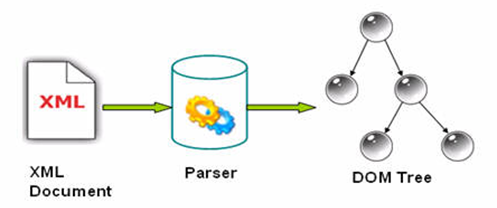
\includegraphics[width=0.5\textwidth]{parsing_xml_to_dom.png}\\[1cm]
%source : http://www.amfastech.com/2014/11/complete-tutorial-on-selecting-best-xml-parser.html
\caption{Parsing d'un document XML en DOM}
\label{Parsing d'un document XML en DOM}
\end{figure}


\subsection{Construction des objets intermédiaires}

Le graphe DOM est ensuite parcouru pour récupérer les différentes informations sur le morceau. Elles seront intégrées dans un arbre d'objets intermédiaires.
\par
Un morceau est composé de plusieurs voix et/ou plusieurs systèmes de voix et a un certain tempo. Un système de voix est constitué de voix. Un tempo a un nombre de battement pas minute et un type de note. Par exemple, le tempo "60 à la noire" signifie qu'il y a 60 noires à la minute, or une noire dure un temps, donc ce tempo est à un temps par seconde.
\par
Une voix est constituée de mesures. Une mesure est composée d'une clé, d'un chiffrage de la mesure et d'une liste d'accords. Un accord a une certaine durée et est composé d'un silence ou d'une liste de notes. Une note a une hauteur et une force (pianissimo, fortissimo, ...).
\par
Le chiffrage de la mesure contient un numérateur, représentant le nombre de temps de la mesure, et un dénominateur, représentant la durée d’une mesure. Une clé contient un nom et un numéro de ligne.


\subsection{Construction des arbres rythmiques}

Les objets intermédiaires sont ensuite utilisés pour construire les arbres rythmiques. Une mesure correspond à un arbre rythmique.



%Un morceau est composé de plusieurs portées et/ou plusieurs systèmes de portée.
%\par
%Un système de portée est constitué de portées.
%\par
%Une porté est liée à un instrument et est composée d’une clé, d’une armure, d’un chiffrage de la mesure et de mesures.
%\par
%Une clé contient un nom et un numéro de ligne.
%\par
%Une armure est composée d'un nombre entier relatif. S'il est négatif alors l'armure contient des bémols, s'il est positif alors elle contient des dièses, s'il vaut 0 alors rien n'est affiché.
%\par
%Le chiffrage de la mesure contient un numérateur, représentant le nombre de temps de la mesure, et un dénominateur, représentant la durée d’une mesure.
%\par
%Une mesure est composée d'une clé optionnelle, d'un chiffrage de la mesure optionnel, de notes, de notes reliées par une division artificielle du temps (duolet/triolet/quartolet/...), d'accords, de silences, de notes reliées par une liaison, de signes indiquant si la mesure est répétée et comment et de notes jouées en crescendo / decrescendo.
%\par
%Une note est constituée d'un nom, d'une série, d'une durée, d'une proportion par rapport à la ronde, d'un point indiquant si elle est pointée ou pas, d'un volume, de paroles et d'une altération (bémol, dièse ou remise à la normal).
%\par
%Un silence est composé d'un nom, d'une série, d'une durée, d'une proportion par rapport à la ronde et d'un point indiquant si elle est pointée ou pas.

%Récapitulatif sous forme de liste:\\
%\begin{itemize}
%\item morceau : plusieurs portées et/ou plusieurs systèmes de portée
%\item système de portée : portées
%\item une porté est lié à un instrument et est composée d’une clé, d’une armure, d’un chiffrage de la mesure et de mesure
%\item clé : nom et numéro de ligne
%\item armure : nombre entier relatif, négatif : bémol, positif : dièse
%\item chiffrage de la mesure : numérateur représentant le nombre de temps de la mesure et dénominateur représentant la durée d’une mesure
%\item mesure : clé optionnelle, chiffrage de la mesure optionnel, notes, notes reliées par une division artificielle du temps (duolet/triolet/quartolet/...), accords, silences, notes reliées par une liaison, si la mesure est répétée et comment, notes jouées en crescendo / decrescendo
%\item note : nom, série, durée, proportion par rapport à la ronde, pointée ou pas, volume, paroles, altération (bémol, dièse ou normal), tiret
%\item silence : nom, série, durée, proportion par rapport à la ronde, pointée ou pas
%\end{itemize}